\documentclass[fleqn,a4paper,12pt]{article}
\usepackage{standalone}		% Zum Einlesen aus anderen .tex-Files
\usepackage{geometry}		% Zur Bearbeitung des Layouts (Ränder,...)
\geometry{left=30mm, right=40mm, bottom=30mm}
\usepackage[german]{babel}
\usepackage[utf8]{inputenc}
\usepackage{amsmath}		% Mathematische Symbole
\usepackage{amssymb}     	% Nochmehr mathematische Symbole
\usepackage{dsfont}      	% Schriftsatz fuer Zahlenmengensymbole
%\usepackage{verbatim}   	% erweiterte Verbatim-Umgebung
\usepackage{alltt}       	% Quasi-Verbatim-Umgebung
\usepackage{fancyhdr}    	% Eigene Kopfzeilen
\usepackage{graphicx}    	% Zum Einbinden von Grafiken
% Einbinden einer eps-Grafik geht so: includegraphics{path}
\usepackage{wrapfig}
\usepackage{lscape}
\usepackage{rotating}
\usepackage{epstopdf}

% Skalierung der Grafiken
\setlength{\unitlength}{1cm}

\pagestyle{fancy}            % Eigene Kopfzeilen verwenden
\frenchspacing               % Kein Extrafreiraum nach Satzzeichen
\setlength{\parindent}{0pt}  % Neue Absaetze nicht einruecken
%\sloppy                     % Schlampige Absatzformatierung
\fussy                       % Penible Absatzformatierung
\linespread{1.5}             % Zeilenabstand

%andere Definitionen
\newcommand{\R}{{\mathbb R}}
\newcommand{\N}{{\mathbb N}}
\newcommand{\Z}{{\mathbb Z}}
\newcommand{\Q}{{\mathbb Q}}
\newcommand{\C}{{\mathbb C}}
\newcommand{\F}{\mathcal{F}}
\newcommand{\less}{\setminus}
\newcommand{\inv}{{}^{-1}}
\newcommand{\Land}{\bigwedge}
\newcommand{\Lor}{\bigvee}

\begin{document}
	"Ubungsaufgabe 9: \newline
	\begin{sidewaysfigure}
		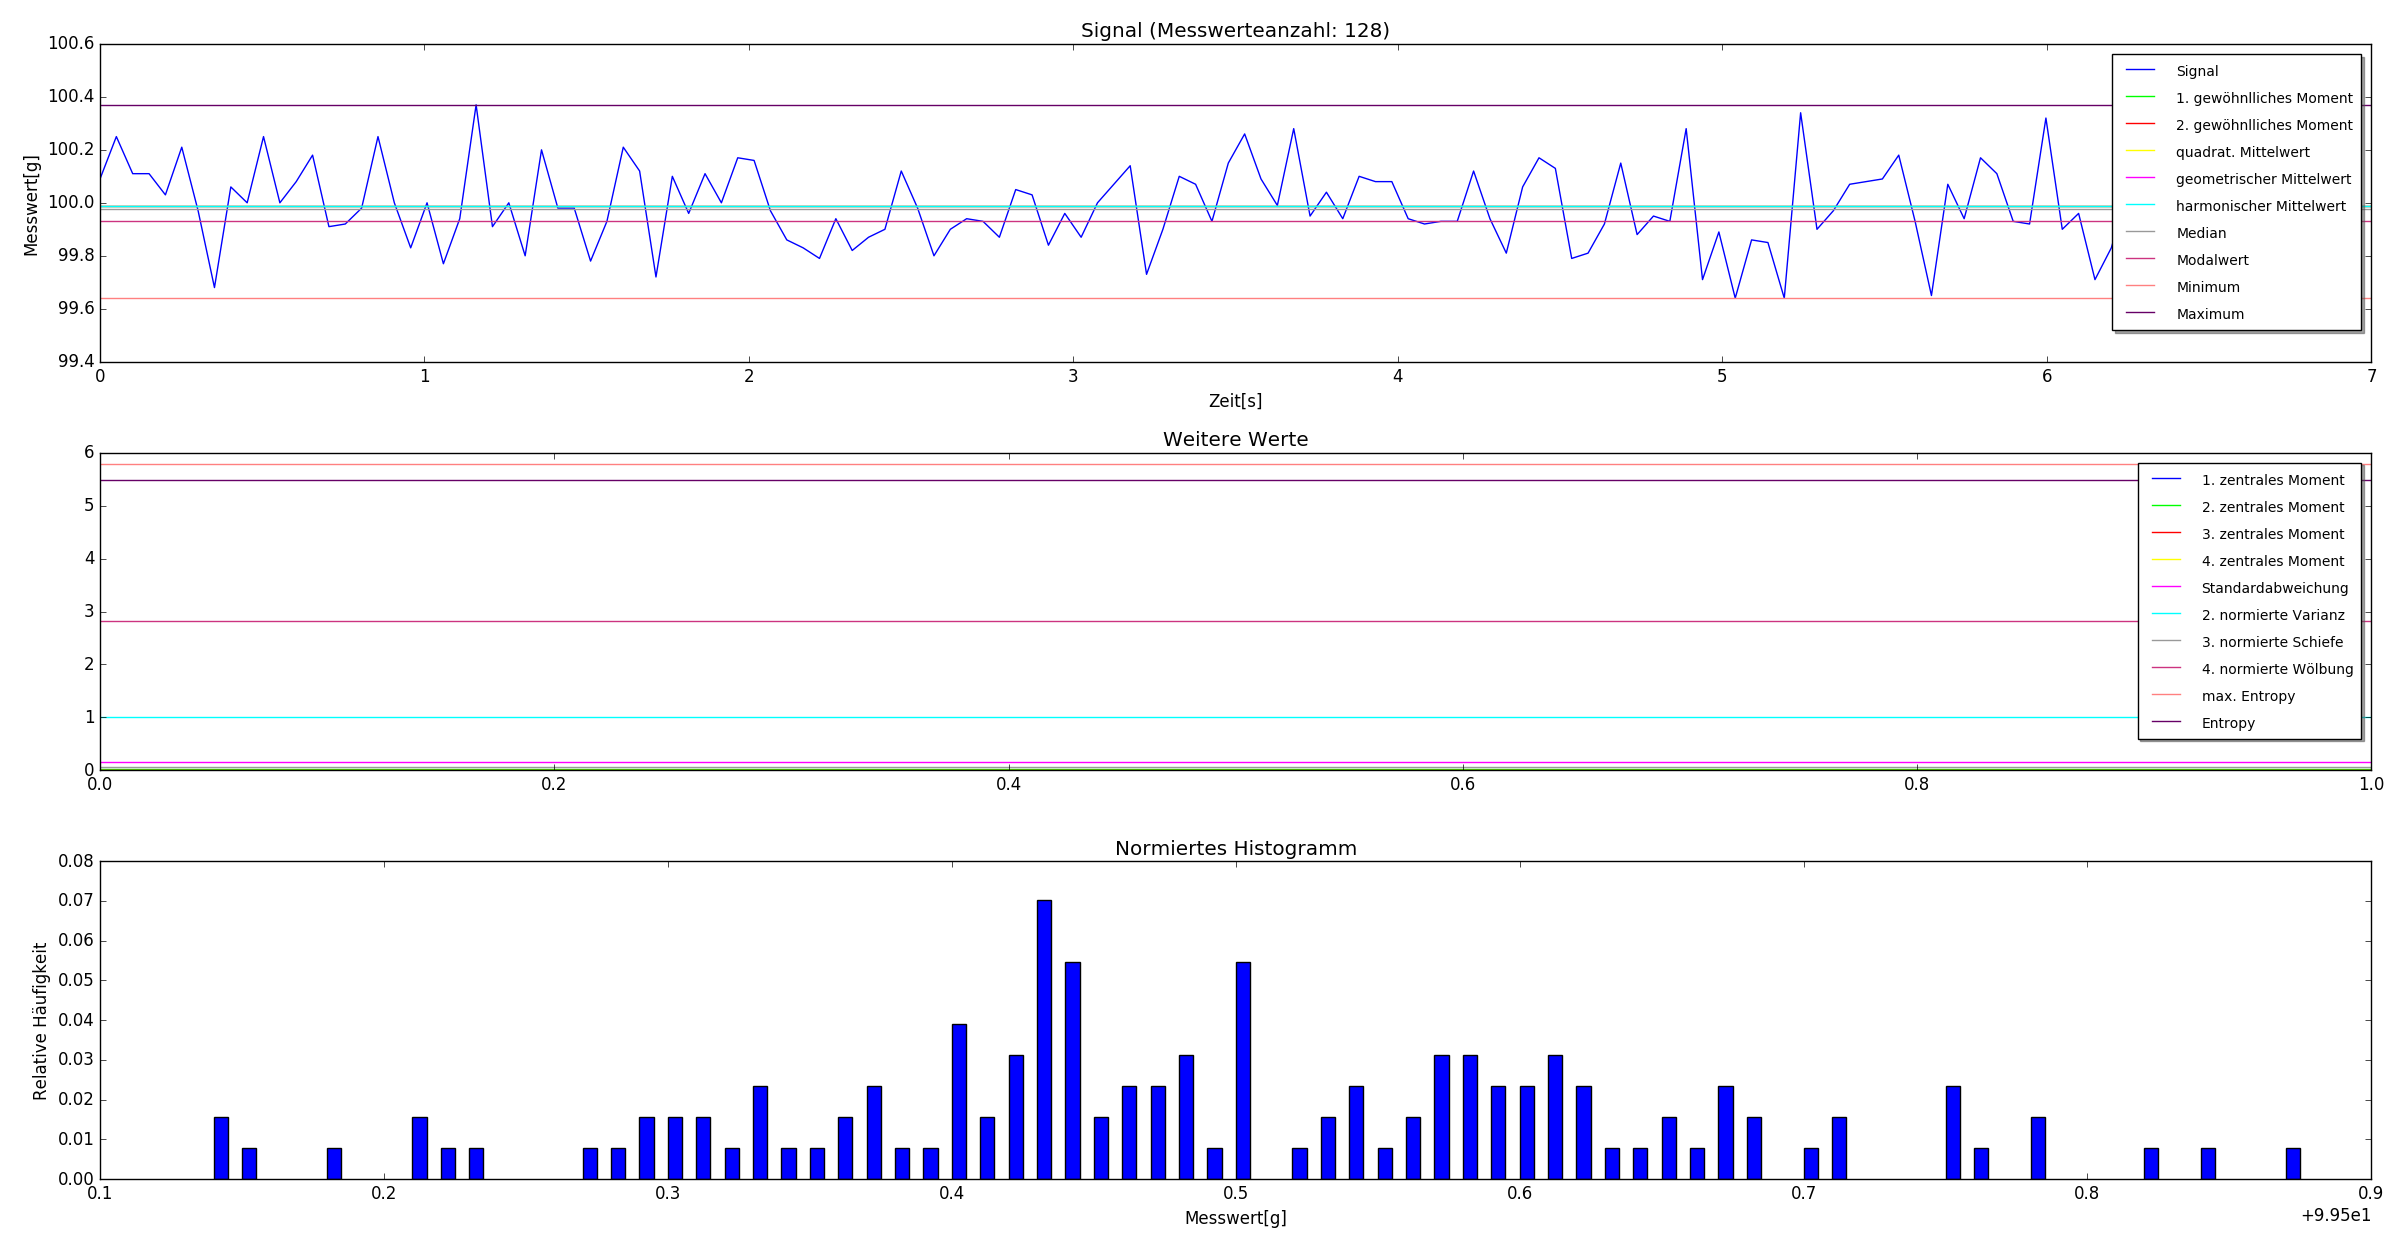
\includegraphics[width=1.0\textwidth]{A09_128.png}
		\caption{(9) Messreihe mit 128 Messwerten}
	\end{sidewaysfigure}
	\begin{sidewaysfigure}
		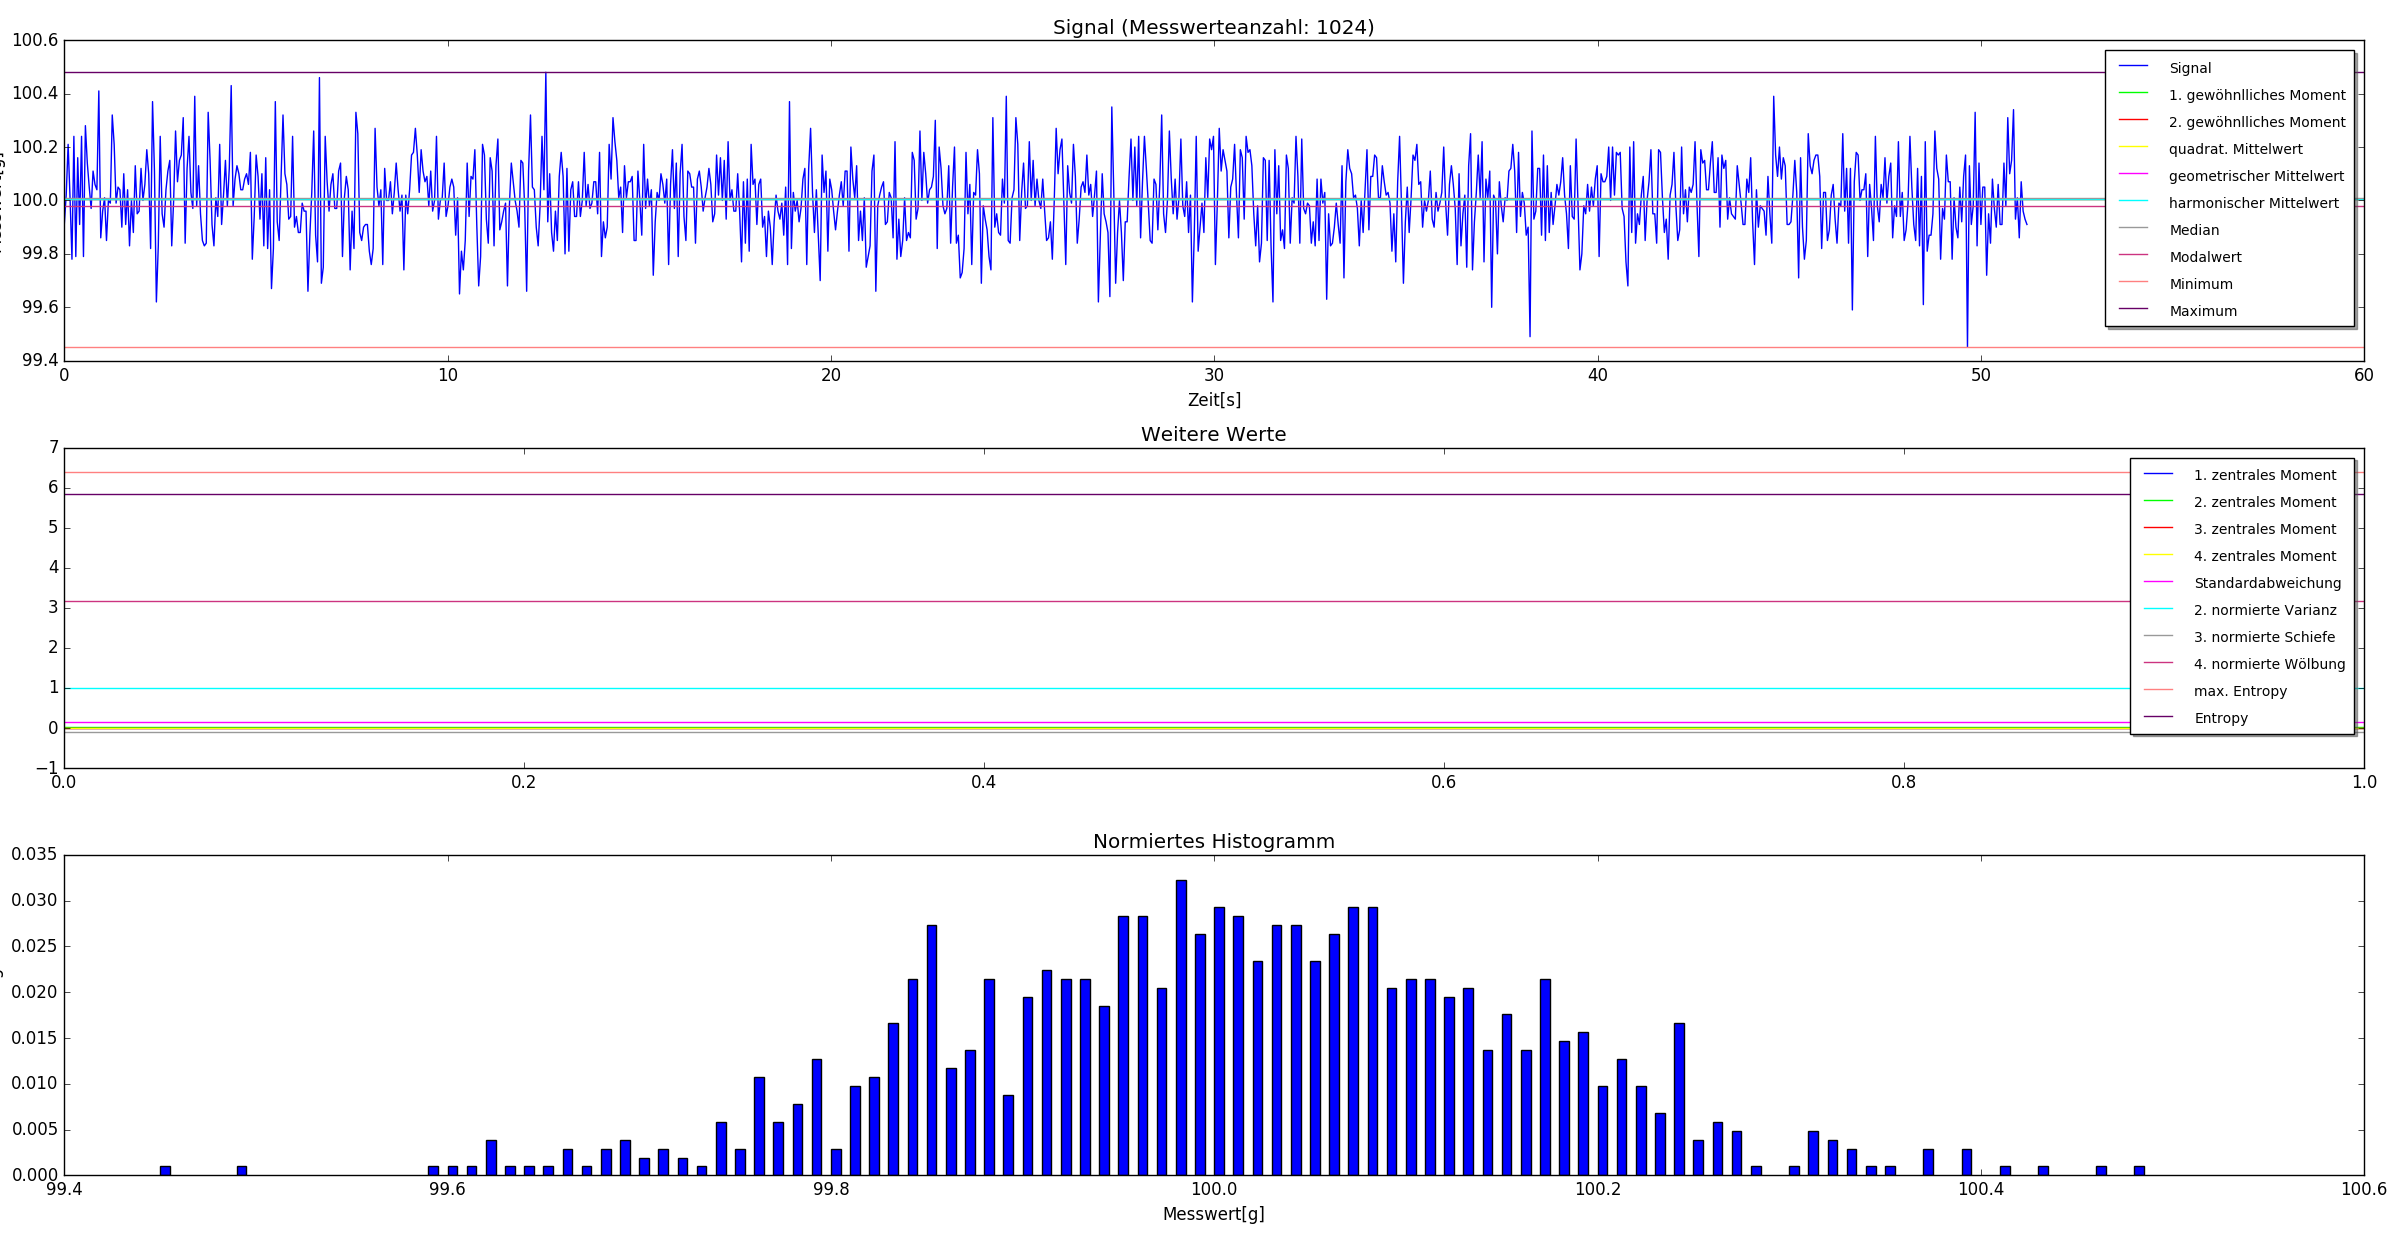
\includegraphics[width=1.0\textwidth]{A09_1024.png}
		\caption{(9) Messreihe mit 1024 Messwerten}
	\end{sidewaysfigure}
	Zur Messreihe mit 1024 Messwerten: \newline
	Mittelungleichung von Cauchy erfüllt: ja \newline
	Normalverteilt: ja \newline
	Interpretation Entropie: Der mittlere Informationsgehalt (Entropie) liegt mit $\approx 5.9$ relativ nah am maximalen Informationsgehalt $\approx 6.4$ (max. Entropie).
	Damit ist der Informationsgehalt eines Messwertes relativ groß.
\end{document}